% !TEX TS-program = XeLaTeX
\documentclass[BScThesis, onesided]{thesis}

\usepackage[colorlinks=true]{hyperref}
\usepackage{amssymb, amsthm, amssymb}
\setcounter{chapter}{1}

%%%%%%%%%%%%%%%%%%%%%%%%%%%%%%%%%%%%%%%%%%%%%%%%%%
%% Add you packages here:

\usepackage{ptext} % Prints text from Shahnameh





%%%%%%%%%%%%%%%%%%%%%%%%%%%%%%%%%%%%%%%%%%%%%%%%%%%
% Bidi packages and fonts:

\usepackage[extrafootnotefeatures]{xepersian}
\settextfont[Scale=1,ExternalLocation=fonts/, BoldFont={HM_FElmiBd}]{HM_FElmi}
\setdigitfont[ExternalLocation=fonts/]{Yas.ttf}
\setcounter{tocdepth}{1} % Dont show sub subsections in ToC.
\renewcommand{\bibname}{مراجع} % Change "Ketabname" to "Maraje"





%%%%%%%%%%%%%%%%%%%%%%%%%%%%%%%%%%%%%%%%%%%%%%%%%%%
% Env definitions (add your own here):

\newtheorem{theorem}{قضیه}[chapter]
\newtheorem{definition}[theorem]{تعریف}
\newtheorem{notation}[theorem]{قرارداد}
\newtheorem{proposition}[theorem]{گزاره}
\newtheorem{lemma}[theorem]{لم}
\newtheorem{remark}[theorem]{تذکر}
\newtheorem{example}[theorem]{مثال}



%%%%%%%%%%%%%%%%%%%%%%%%%%%%%%%%%%%%%%%%%%%%%%%%%%%
% Command definitions (add your own here):

\newcommand{\E}{\mathbb{E}}
\newcommand{\N}{\mathcal{N}}
\newcommand{\Prob}{\mathbb{P}}
\newcommand{\bfphi}{\bm {\phi}}
\newcommand{\mubf}{\bm \mu}
\newcommand{\Ybf}{\bm Y}
\newcommand{\Hc}{\mathcal{H}}
\newcommand{\bx}{\mathbf{x}}
\newcommand{\R}{\mathbb{R}}
\newcommand{\Nd}{\mathcal{N}}
\newcommand{\tr}{\mathrm{tr}}
\newcommand{\HSIC}{\mathrm{HSIC}}
\newcommand{\LL}{\mathcal{L}}
\newcommand{\bigCI}{\mathrel{\text{\scalebox{1.07}{$\perp\mkern-10mu\perp$}}}}

%%%%%%%%%%%%%%%%%%%%%%%%%%%%%%%%%%%%%%%%%%%%%%%%%%%%%%%%%%%%%%%%%%%%%%%%%%%%%%%%%%%%%%%%%%%%%%%%%%%%%%
%%%%%%%%%%%%%%%%%%%%%%%%%%%%%%%%%%%%%%%%%%%%%%%%%%%%%%%%%%%%%%%%%%%%%%%%%%%%%%%%%%%%%%%%%%%%%%%%%%%%%%
%%%%%%%%%%%%%%%%%%%%%%%%%%%%%%%%%%%%%%%%%%%%%%%%%%%%%%%%%%%%%%%%%%%%%%%%%%%%%%%%%%%%%%%%%%%%%%%%%%%%%%

\begin{document}

%%%%%%%%%%%%%%%%%%%%%%%%%%%%%%%%%%%%%%%
% Title/Author/...

\logo{
\includegraphics{logo}}
\date{\vspace{0.8cm}
	تابستان ۱۳۹۹
}
\title{\LARGE
عنوان پروژه‌ی کارشناسی 
}
\author{نام نام‌خانوادگی}
\consult{دکتر محمد محمدی}
\university{دانشگاه صنعتی شریف\\دانشکده‌ی مهندسی برق}
\subject{مهندسی برق گرایش سیستم‌ها و شبکه‌های مخابراتی}
\supervisor{دکتر قاسم قاسم‌نژاد}
\frontmatter
\makethesistitle \pagestyle{empty} \baselineskip1.1\baselineskip


%%%%%%%%%%%%%%%%%%%%%%%%%%%%%%%%%%%%%%%
% acknowledgements

\begin{قدردانی}
از آقای فلانی به خاطر راهنمایی‌های ارزشمندشان در رابطه با بهمان کار، سپاس‌گزارم. 
این پروژه، بدون راهنمایی‌های ایشان هرگز به سرانجام نمی‌رسید.
\end{قدردانی}

%%%%%%%%%%%%%%%%%%%%%%%%%%%%%%%%%%%%%%%
% abstract

\begin{abstract}
{کلمه کلیدی اول، کلمه کلیدی دوم، کلمه کلیدی سوم} 
این پروژه، چکیده مشخصی ندارد.
\end{abstract}

%%%%%%%%%%%%%%%%%%%%%%%%%%%%%%%%%%%%%%%
%  Printing tables of contents

\pagestyle{plain}\pagenumbering{tartibi}\tableofcontents\listoffigures
~~
\paragraphfootnotes %Make footnotes in line
\pagenumbering{arabic}

%%%%%%%%%%%%%%%%%%%%%%%%%%%%%%%%%%%%%%%

\chapter{نمونه‌ی فصل}

\ptext

\section{نمونه‌ی تصویر}

در این بخش، یک نمونه‌ی تصویر را می‌بینید.

\begin{figure}[h!]
    \centering
    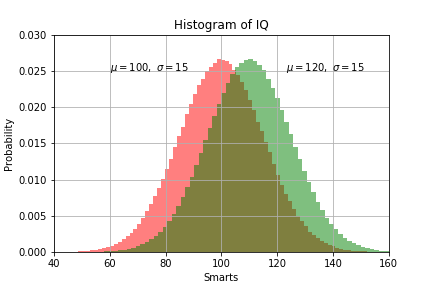
\includegraphics[width=0.8\textwidth]{save.png}
    \caption{یک نمونه کپشن برای عکس.}
    \label{fig:my_label}
\end{figure}


\section{نمونه‌ی فرمول}

در این بخش به مطالعه‌ی متغیّرهای زیر--گوسی می‌پردازیم. هدف آوردن چند نمونه‌ی فرمول در این فایل است.

	\subsection{متغیّرهای تصادفی زیر--گوسی}
	\begin{definition}
		متغیّر تصادفی
		\lr{$X$}
		با میانگین
		\lr{$\mu = \mathbb{E}[X]$}
		را زیر--گوسی می‌نامیم هرگاه عدد مثبتی مانند
		\lr{$\sigma$}
		وجود داشته باشد، به قسمی که برای هر
		\lr{$\lambda\in\mathbb{R}$}
		داشته باشیم
		\[\E\left[e^{\lambda(X-\mu)}\right]\leq e^{\frac{\sigma^2\lambda^2}{2}}.\]
	\end{definition}
	ثابت
	\lr{$\sigma$}
	را پارامتر این متغیّر تصادفی می‌نامیم. به عنوان مثال، یک متغیّر تصادفی گوسی با واریانس
	\lr{$\sigma^2$}،
	خود یک متغیّر تصادفی زیر--گوسی با پارامتر
	\lr{$\sigma$}
	است. هم‌چنین تعداد زیادی از متغیّرهای تصادفی غیر گوسی، زیر--گوسی هستند.
	
	\begin{theorem}	\label{thm1subgaussian}
		برای هر متغیّر تصادفی زیر--گوسی 
		\lr{$X$}
		با متوسّط
		\lr{$\mu = \E[X]$}
		و پارامتر
		\lr{$\sigma$}
		داریم
		\begin{equation}
		\Prob[|X-\mu|\geq t] \leq 2e^{-\frac{t^2}{2\sigma^2}}.
		\end{equation}
	\end{theorem}
	\begin{proof}
		از نامساوی مارکف می‌دانیم
		\[\Prob[X-\mu\geq t] = \Prob[e^{\lambda (X-\mu)} \geq e^{\lambda t}] \leq \frac{\E\left[e^{\lambda (X-\mu)}\right]}{e^{\lambda t}}. \]
		حال با توجّه به تعریف متغیّرهای تصادفی زیر--گوسی داریم
		\[\Prob[X-\mu\geq t] \leq \frac{\E\left[e^{\lambda (X-\mu)}\right]}{e^{\lambda t}} \leq \exp(\frac{\sigma^2\lambda^2}{2} - \lambda t).\]
		نامساوی بالا به ازای هر
		\lr{$\lambda\in\R$}
		برقرار است، من‌جمله
		\lr{$\lambda$}ای
		که طرف راست را کمینه کند. در نتیجه
		\begin{equation}
		\Prob[X-\mu\geq t] \leq \inf_\lambda\left\{\exp(\frac{\sigma^2\lambda^2}{2} - \lambda t) \right\} = e^{-\frac{t^2}{2\sigma^2}}.
		\end{equation}
		همچنین اگر متغیّر تصادفی
		\lr{$X$}،
		زیر--گوسی باشد، 
		\lr{$-X$}
		هم زیر--گوسی است و به طور مشابه، داریم
		\[\Prob[-X+\mu\geq t] = \Prob[X-\mu\leq -t]\leq  e^{-\frac{t^2}{2\sigma^2}}\]
		و می‌توان نوشت
		\[\Prob[|X-\mu|\geq t] \leq \Prob[X-\mu\geq t] + \Prob[X-\mu\leq -t] \leq 2e^{-\frac{t^2}{2\sigma^2}}.\]
		
	\end{proof}
	
	متغیّرهای تصادفی زیر--گوسی خواصّ گوناگونی دارند، تعدادی از این خواص را در قضایای بعدی مشاهده می‌کنیم.
	
	\begin{theorem}\label{thm2subgaussian}
		فرض کنید 
		\lr{$X$}
		یک متغیّر تصادفی زیر--گوسی با امید ریاضی
		\lr{$\E[X]=0$}
		باشد، در این صورت اگر متغیّر تصادفی 
		\lr{$Z$}
		را به صورت
		\lr{$Z\sim \Nd(0,2\sigma^2)$}
		در نظر بگیریم، داریم
		\begin{equation}
		\Prob[|X|\geq s] \leq \sqrt{8}e \Prob[|Z|\geq s] \qquad \forall s \geq 0.
		\label{thm2eq}
		\end{equation}
	\end{theorem}
	\begin{proof}
		از قضیه‌ی
		\ref{thm1subgaussian}
		داریم:
		\[\Prob[X\geq t] \leq e^{-\frac{t^2}{2\sigma^2}}\qquad \forall t\geq0\]
		و از طرف دیگر، با توجّه به کران
		\lr{Mills ratio}
		برای توزیع‌های گوسی داریم
		\[\Prob[Z\geq t] \geq\left(\frac{\sqrt{2}\sigma}{t} - \frac{(\sqrt{2}\sigma)^3}{t^3} \right) e^{-\frac{t^2}{4\sigma^2}}.\]
		حال دو حالت زیر را در نظر می‌گیریم:	
		حالتی که 
		\lr{$t\in[0,2\sigma]$}
		باشد. در این حالت، داریم
		\[\Prob[Z\geq t] \geq \Prob[Z\geq 2\sigma] = \left(\frac{1}{\sqrt{2}} - \frac{1}{2\sqrt{2}} \right) e^{-1} = \frac{1}{\sqrt{8}e}\]
		و از آن‌جا که
		\lr{$\Prob[X\geq t] \leq 1$}،
		داریم
		\[\frac{\Prob[X\geq t]}{\Prob[Z\geq t]} \leq \sqrt{8}e.\]
		
		
		حالتی که
		\lr{$t>2\sigma$}
		باشد. در این حالت اگر کران
		\lr{Mills ratio}
		را با کران به دست آمده در قضیه‌ی
		\ref{thm1subgaussian}
		ترکیب کنیم و تعریف کنیم
		\lr{$s = \frac{t}{\sigma}$}،
		داریم
		\begin{flalign*}
		\sup_{t>2\sigma} \frac{\Prob[X\geq t]}{\Prob[Z\geq t]} &\leq \sup_{s>2}\frac{e^{-\frac{s^2}{4}}}{\frac{\sqrt{2}}{s} - \frac{2\sqrt{2}}{s^3}}\\
		&\leq \sup_{s>2} s^3 e^{-\frac{s^2}{4}}\\
		&\leq \sqrt{8}e.
		\end{flalign*}
		پس در هر دو حالت نامساوی
		(\ref{thm2eq})
		برقرار است.		
	\end{proof}
	
\section{نمونه‌ی ارجاع}

در این بخش، یک نمونه ارجاع را خواهیم دید.

\subsection{شرایط لازم مرتبه‌ی اول و مرتبه‌ی دوم }

در ابتدا به بیان قضیه‌ی معروف شرایط لازم، در بهینه‌سازی غیرمحدب می‌پردازیم. 
\begin{theorem}
یک مسئله‌ی بهینه‌سازی مقید غیرمحدّب را به فرم
$\min_{h(W) = 0} f(W)$
را در نظر بگیرید، که در آن
$f: \R^{d\times q} \to \R$
و
$h: \R^{d\times q} \to \R^{q\times q}$
توابعی دو بار مشتق‌پذیر با مشتق پیوسته بوده و 
$\LL$
لاگرانژین این مسئله‌ی بهینه‌سازی باشد. آن‌گاه، برای هر بهینه‌ی محلّی،  ماتریس
$\Lambda^*$
وجود دارد که  در شرایط زیر صدق می‌کند:
\begin{itemize}
\item
شرط
\lr{KKT}:
\begin{equation}
\nabla_W \LL(W^*, \Lambda^*) =0 \;\;\;\;\;
\nabla_\Lambda \LL(W^*, \Lambda^*) =0.
\end{equation}

\item
شرایط لازم مرتبه‌ی دوم:
\begin{equation}
\tr (Z^\top \nabla^2_{WW} \LL (W^*, \Lambda^*)Z) \geq 0 \;\; \forall Z\neq 0 \;\;\;  \mathrm{with} \;\;\; \nabla h(W^*)^\top Z = 0.
\end{equation}
\end{itemize}
\end{theorem}
\begin{proof}
	اثبات این قضیه در اکثر کتاب‌های بهینه‌سازی غیرمحدّب موجود است. به عنوان مثال 
	\cite{nocedal2006numerical}
	را ببینید.
\end{proof}


\chapter{جمع‌بندی}

در این پروژه، به بررسی نتایج تئوری و تلاش‌های موجود برای اثبات قضیه‌ی جدایی‌پذیری مخلوط‌های غیرخطی فرآیند‌های تصادفی خطی و غیرخطی پرداختیم. نشان دادیم که در حالت کلّی، جداسازی مخلوط‌های غیرخطی غیرممکن است و مثال‌هایی از مسائل غیرخطی معرفی کردیم که در آن‌ها مخلوط‌های غیرخطی جدایی‌پذیر نیستند. بعد از مرور الگوریتم‌های کمینه‌سازی اطلاعات متقابل و کاربرد‌های آن‌ها در جداسازی مخلوط‌های خطی، الگوریتمی مشابه برای جداسازی مخلوط‌های غیرخطی ارائه و عملکرد تجربی این الگوریتم را بررسی نمودیم. در انتها به مطالعه‌ی مخلوط‌های غیرخطی فرآیند‌های تصادفی گوسی و ارائه‌ی الگوریتم‌هایی برای جداسازی این مخلوط‌ها پرداختیم و الگوریتم‌ها را نیز از نظر کارکرد با یکدیگر مقایسه کردیم.


\bibliography{bib}
\bibliographystyle{ieeetr-fa}

\end{document}